%\VignetteIndexEntry{Integrated Species Distribution Models}
%\VignettePackage{RISDM}
%\VignetteEngine{knitr::knitr}

\documentclass[article,shortnames,nojss]{jss}\usepackage[]{graphicx}\usepackage[]{xcolor}
% maxwidth is the original width if it is less than linewidth
% otherwise use linewidth (to make sure the graphics do not exceed the margin)
\makeatletter
\def\maxwidth{ %
  \ifdim\Gin@nat@width>\linewidth
    \linewidth
  \else
    \Gin@nat@width
  \fi
}
\makeatother

\definecolor{fgcolor}{rgb}{0.345, 0.345, 0.345}
\newcommand{\hlnum}[1]{\textcolor[rgb]{0.686,0.059,0.569}{#1}}%
\newcommand{\hlstr}[1]{\textcolor[rgb]{0.192,0.494,0.8}{#1}}%
\newcommand{\hlcom}[1]{\textcolor[rgb]{0.678,0.584,0.686}{\textit{#1}}}%
\newcommand{\hlopt}[1]{\textcolor[rgb]{0,0,0}{#1}}%
\newcommand{\hlstd}[1]{\textcolor[rgb]{0.345,0.345,0.345}{#1}}%
\newcommand{\hlkwa}[1]{\textcolor[rgb]{0.161,0.373,0.58}{\textbf{#1}}}%
\newcommand{\hlkwb}[1]{\textcolor[rgb]{0.69,0.353,0.396}{#1}}%
\newcommand{\hlkwc}[1]{\textcolor[rgb]{0.333,0.667,0.333}{#1}}%
\newcommand{\hlkwd}[1]{\textcolor[rgb]{0.737,0.353,0.396}{\textbf{#1}}}%
\let\hlipl\hlkwb

\usepackage{framed}
\makeatletter
\newenvironment{kframe}{%
 \def\at@end@of@kframe{}%
 \ifinner\ifhmode%
  \def\at@end@of@kframe{\end{minipage}}%
  \begin{minipage}{\columnwidth}%
 \fi\fi%
 \def\FrameCommand##1{\hskip\@totalleftmargin \hskip-\fboxsep
 \colorbox{shadecolor}{##1}\hskip-\fboxsep
     % There is no \\@totalrightmargin, so:
     \hskip-\linewidth \hskip-\@totalleftmargin \hskip\columnwidth}%
 \MakeFramed {\advance\hsize-\width
   \@totalleftmargin\z@ \linewidth\hsize
   \@setminipage}}%
 {\par\unskip\endMakeFramed%
 \at@end@of@kframe}
\makeatother

\definecolor{shadecolor}{rgb}{.97, .97, .97}
\definecolor{messagecolor}{rgb}{0, 0, 0}
\definecolor{warningcolor}{rgb}{1, 0, 1}
\definecolor{errorcolor}{rgb}{1, 0, 0}
\newenvironment{knitrout}{}{} % an empty environment to be redefined in TeX

\usepackage{alltt}

%% almost as usual
\author{Scott D. Foster\\Data61, CSIRO, Hobart, Tasmania, Australia}
\title{An Introduction to \pkg{RISDM}}
\date{\itshape\today}

%% for pretty printing and a nice hypersummary also set:
\Plainauthor{Scott D. Foster} %% comma-separated
\Plaintitle{An Introduction/Tutorial to RISDM} %% without formatting
\Shorttitle{RISDM} %% a short title (if necessary)

\Abstract{
Species distribution models (SDMs) describe the distribution of a species through space, environment and possibly time. They are based on two types of data input: those that inform the biology of where the species is found (and possibly isn't), and those that describe the environment throughout the study region. An SDM is formed by describing the variation in the species data in terms of the variation in the environmental data (a correlative model). SDMs are a useful and proven tool for science and management. 

Standard implementations of SDMs requires a possibly over-restrictive homogeneity in sources of biological data. Typically, the biological data is one of: presence-only (PO), presence-absence (PA), or abundance (AA) data. Results from SDMs using single sources of data will suffer from inherent biases and limitations to that data type. For example, PO data contains observer-bias and presence-absence (PA) and abundance (AA) data is often less geographically expansive and of limited quantity (and hence information content).

Intuitively, it is appealing to incorporate as much biological information into the SDM as possible. This means that multiple data sources and multiple data types should be integrated in a single model. This is the central idea that \textit{integrated} SDMs, or ISDMs, bring \citep{fle19,mil19,isa20}. However, the structure of ISDMs is a necessary step-change in complexity to single data source SDMs -- the vagueries of the each contirbuting data sets need to be modelled as well as the differences between data sets. In addition, there are statistical specifications that need to be handled as well, such as handling multiple likelihoods in a single model.

The \proglang{R}-package \texttt{RISDM} provides a task-specific tool for fitting ISDMs. RISDM utilises the computational engine of \texttt{INLA} \citet{rue09} as the back end, but hides the \texttt{INLA}-specific details from the user (such as the creation of stacks, the specification of spatial models and the specification of multiple likelihoods). The \texttt{RISDM} interface is simplified as much as possible, but still remains flexible enough for a wide class of models to be fitted. In particular, the workflow is purposefully designed to follow that of a \texttt{glm} or \texttt{gam}: model fit, model diagnostics, model summary/interpretation, and prediction.

In this document, we illustrate the process of fitting an ISDM to an invasive weed data set from northern Australia. We illustrate the steps of analysis, and show the effect of altering some of the main parameters/options/control.
}
\Keywords{Integrated Species Distribution Models, ISDM, INLA, SPDE, \proglang{R}}
\Plainkeywords{Integrated Species Distribution Models, ISDM, INLA, SPDE, R} %% without formatting

\Address{
  Scott D. Foster\\
  Data61, CSIRO\\
  Marine Laboratories\\
  GPObox 1538\\
  Hobart 7001\\
  Australia
  E-mail: \email{scott.foster@data61.csiro.au}
}

\usepackage{natbib}
\usepackage{url}
\usepackage{hyperref}
\usepackage{color}

\renewcommand{\thefootnote}{\fnsymbol{footnote}}
\IfFileExists{upquote.sty}{\usepackage{upquote}}{}
\begin{document}

\footnotetext{This is an introduction to the RISDM R-pacakge (available from \url{https://cran.r-project.org/package=RISDM}).}

%<<prelim, echo = FALSE, results = "hide">>=


\section*{First Things First (setting up R for using \texttt{RISDM})}

Before starting with this introduction to \texttt{RISDM}, we need to make sure that everything is set up properly. Much of this will vary from computer to computer, but you must have a working version of R installed (preferably the recent release) and a working version of INLA \citep{rue09}. This vignette was created using R-version R version 4.2.1 (2022-06-23), \texttt{INLA} release 23.04.24, and \texttt{RISDM} release 1.2.7. It does not matter whether you prefer to use R through a development environment (such as RStudio) or through the command line -- the results will be the same. You will need to have installed a recent version of \texttt{INLA} and \texttt{RISDM}. These can be installed by starting R and then submitting (at command line):
\begin{knitrout}
\definecolor{shadecolor}{rgb}{0.969, 0.969, 0.969}\color{fgcolor}\begin{kframe}
\begin{alltt}
\hlkwd{install.packages}\hlstd{(}\hlstr{"INLA"}\hlstd{,}\hlkwc{repos}\hlstd{=}\hlkwd{c}\hlstd{(}\hlkwd{getOption}\hlstd{(}\hlstr{"repos"}\hlstd{),}
                \hlkwc{INLA}\hlstd{=}\hlstr{"https://inla.r-inla-download.org/R/stable"}\hlstd{),} \hlkwc{dep}\hlstd{=}\hlnum{TRUE}\hlstd{)}
\hlcom{#vignette not built to save computation}
\hlstd{devtools}\hlopt{::}\hlkwd{install_github}\hlstd{(} \hlkwc{repo}\hlstd{=}\hlstr{"Scott-Foster/RISDM"}\hlstd{,} \hlkwc{build_vignettes}\hlstd{=}\hlnum{FALSE}\hlstd{)}
\end{alltt}
\end{kframe}
\end{knitrout}
The \texttt{RISDM} package will then need to be loaded. The raster package is also loaded to handle spatial data.
\begin{knitrout}
\definecolor{shadecolor}{rgb}{0.969, 0.969, 0.969}\color{fgcolor}\begin{kframe}
\begin{alltt}
\hlkwd{library}\hlstd{( RISDM)}
\hlkwd{library}\hlstd{( raster)}
\end{alltt}
\end{kframe}
\end{knitrout}

\section*{Introduction to RISDM, via Example}

The structure and function calls within \texttt{RISDM} are designed to follow that of the \texttt{glm()} and \texttt{gam()} that are part of the well-used \texttt{stats} \citep{R22} and \texttt{mgcv} \citep{woo17} packages respectively. The \texttt{RISDM} approach is designed to broaden the user-base of ISDM models by leveraging off familiar analytical and computational concepts. While very advanced users may want to fit models that are outside of the scope of \texttt{RISDM}, the \texttt{RISDM} framework could still be used to provide many of the constructs needed for lower-level modelling with \texttt{INLA} \citep{rue09}.

This document is structured, more-or-less, to match the steps that an analyst follows in an analysis workflow. At least for an archetypical analysis. That is: 
\begin{enumerate}
  \item \hyperref[subsec:prep]{Preparation} (data and analysis \hyperref[subsubsec:mesh]{mesh})
  \item \hyperref[subsec:mod]{Specifying and Evaluating} (`fitting`) the model
  \item \hyperref[subsubsec:res]{Checking the model} for any obvious departures, and \hyperref[subsubsec:summ]{understanding/summarising} the model.
  \item \hyperref[subsec:pred]{Prediction}
\end{enumerate}

The \texttt{RISDM} package is introduced here using data on gamba grass in the Northern Territory, Australia. These data are a small subset of all those available, and are intended to be an illustrative `toy' -- containing enough complexity to be real, but not so complex that they provide too much distraction from the method and computation. The data are presented in \citet{fos24} and the reader should refer there for some more detail and for references.

\subsection*{Preparation} \label{subsec:prep}

\subsubsection*{Covariate Data -- setting the environmental scene}\label{subsubsec:covs}

The first piece of the data puzzle is the environmental data. These data are assumed to be defined on a raster (from the raster package) and must form a raster brick. Forming them into a raster stack ensures that the individual raster layers all have the same extent and the same resolution etc. It is not necessary, but it is highly recommended, that the analyst considers the pattern of missing values within the raster stack -- where some covariates are available but others are not. Missing values in covariates in any correlative model can substantially reduce the information content.

The covariate data for the gamba grass example is included as part of the \texttt{RISDM} package. There are three raster layers: 
\begin{enumerate}
  \item Accessibility, using the method by \citep{wei18} was used after small modification for the northern Australian context. Here, it measures the travel time to any settlement with a population of more than 200 \citep{geo06}. The observed distribution of this covariate was right-skewed, so a square root transformation was taken. This was to try and reduce the leverage of unusually large observations. One method of spreading gamba grass is thought to be through human movement. So accessibility may correlate with gamba distribution.
  \item Elevation, measured through a digital elevation model \citep[DEM; from][]{gal15}, may delineate gamba grass distribution \citep{ada15}. Like accessibility, a square root transformation was used to endeavour to reduce leverage of unusual locations within the analysis.
  \item Soil moisture at the root zone \citep[SMRZ][]{fro18} may limit gamba grass distribution as it could require moist but not saturated soils \citep{flo05,pet12}.
\end{enumerate}
The gamba grass covariates can be read directly into R and compiled into a raster stack. The distribution of the covariate data has been inspected (elsewhere) and corrective steps have been employed. For the gamba data, the accessibility and the DEM were square-root transformed to reduce skewness of their distributions, which will also lead to reducing the influence in the analysis of very high values. This is to reduce the leverage of these observations and to try and obtain the most amount of reliable information from these data. 
\begin{knitrout}
\definecolor{shadecolor}{rgb}{0.969, 0.969, 0.969}\color{fgcolor}\begin{kframe}
\begin{alltt}
\hlstd{filenames} \hlkwb{<-} \hlkwd{paste0}\hlstd{(} \hlkwd{system.file}\hlstd{(}\hlstr{"extdata"}\hlstd{,} \hlkwc{package}\hlstd{=}\hlstr{"RISDM"}\hlstd{),}
                   \hlkwd{c}\hlstd{(}\hlstr{"/GambaExample_sqrtACC_23Mar28.tif"}\hlstd{,}
                     \hlstr{"/GambaExample_sqrtDEM_23Mar28.tif"}\hlstd{,}
                     \hlstr{"/GambaExample_SMRZ_23Mar28.tif"}\hlstd{))}
\hlstd{covars} \hlkwb{<-} \hlkwd{stack}\hlstd{( filenames)}
\hlkwd{names}\hlstd{( covars)} \hlkwb{<-} \hlkwd{c}\hlstd{(}\hlstr{"ACC"}\hlstd{,}\hlstr{"DEM"}\hlstd{,}\hlstr{"SMRZ"}\hlstd{)}
\hlkwd{print}\hlstd{(} \hlkwd{colnames}\hlstd{(} \hlkwd{coordinates}\hlstd{( covars)))}  \hlcom{#to see how things are labelled.}
\end{alltt}
\begin{verbatim}
[1] "x" "y"
\end{verbatim}
\begin{alltt}
\hlkwd{plot}\hlstd{( covars)}
\end{alltt}
\end{kframe}\begin{figure}

{\centering 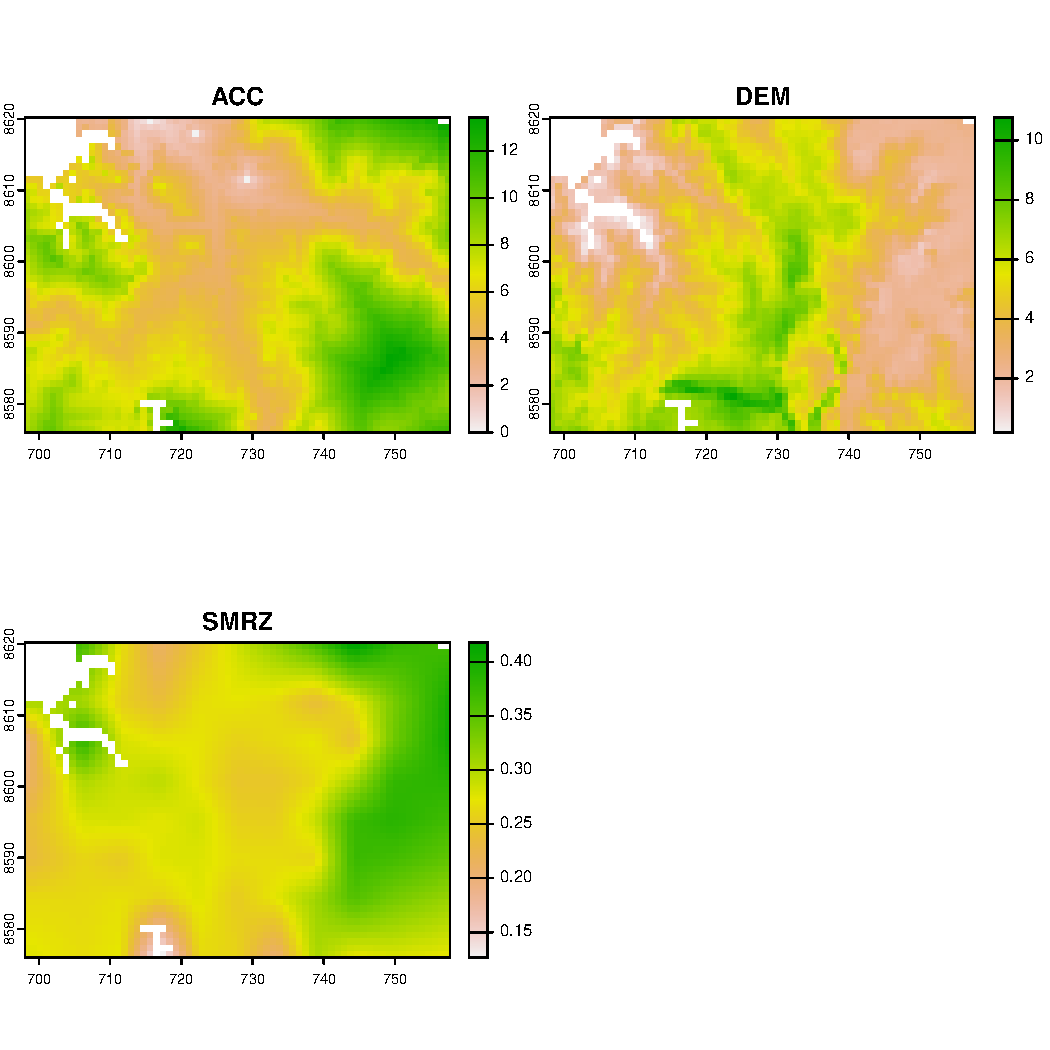
\includegraphics[width=\maxwidth]{figure/readCovars-1} 

}

\caption[Environmental covariate data for the gamba grass example]{Environmental covariate data for the gamba grass example. Accessibility (ACC) measuring effective distance for humans to travel. Digital elevation model (DEM) giving the altitude. Soil moisture at the root zone (SMRZ) measuring the wetness where it matters for plants. See text for details and references.}\label{fig:readCovars}
\end{figure}

\end{knitrout}
It may be that the raster data that an analyst wants to use comes in different resolutions, different projections, different extents and so on. If the analyst is not familiar with conversion of these, then it is suggested that they should look into the \texttt{projectRaster}, \texttt{aggregate}, \texttt{disaggregate}, \texttt{mask}, \texttt{crop} and \texttt{stack} functions from the \texttt{raster} package \citep{hij22}.

For the environmental data in this example (see Figure \ref{fig:readCovars}), we have used an equal area project (UTM zone 52 south) with kilometre map units. We recommend the use of projected rasters, as this eases specification and interpretation of spatial processes. However, \texttt{RISDM} will still work with whatever coordinate reference system is chosen.

The resolution of the raster is used to define the resolution of the underlying point process in the ISDM. It is reasonably argued that performing point-process computation on grids smaller than this is wasteful as environmental conditions would not then change between many neighbouring cells. As the raster defines point process computational scale, it can sometimes be useful -- at the start of a modelling exercise -- to coarsen the resolution just so models run faster.

\subsubsection*{Bias Data}

In addition to the environmental covariates, the raster stack can (and should if available) covariates that could delineate the sampling bias of the PO data \citep[e.g.][]{war13}. That is, covariates that are suspected of describing the pattern of search effort that could then result in a set of presences. For the gamba grass example, the accessibility (ACC) variable is likely to play this delineating role. When there are more than one data type, there is no issue that a single covariate describes both the distribution of the species \textit{and} the search bias.

\subsubsection*{Observation Data}

The observation data are those that inform the where the species is, is not, and in what quantity/abundance. Each type of data (PO, PA or AA) is required to have its own data object. They are all required to have the same projection as the raster stack for the environment. This assumes that the coordinate names are the same too. The observation data sets are:
\begin{description}
  \item[Presence-Only (PO) data] A \texttt{data.frame} containing at least the locations (x and y coordinates) of the presences. The data.frame may also contain extra contextual information, like the survey/database the presence record was recorded in. This contextual information is currently not used in the analysis.
  \item[Presence-Absense (PA) and Abundance (AA) data] A \texttt{data.frame} for PA and a \texttt{data.frame} for AA (separately, but neither \textit{has to be} specified). The data.frames contain at least: 
  \begin{enumerate}
    \item The locations (x and y coordinates) where the observation occurred.
    \item The value of the observation at these locations. For PA data, this is a `0' for an absence and a `1' for a presence. For AA data, this is a positive integer (or zero).
    \item The geographical area (sample area) that the sampling method searched to record the observation. Intuitively, a search area of 1m$^2$ is more likely to produce a `0' than a search area of 1000m$^2$. If sample area is unknown then it must be either guessed (!?) or have some constant inputed. In either case, the results are unlikely to then be reflective of overall levels of species abundance, but the distribution \textit{may very well be} relative to the actual distribution.
    \item (optional) Extra information that could explain variation in the PA or AA data. Such information could include data that might induce heterogeneous detectability (e.g. different sampling tools, different operators, and so on), but it may also include continuous variables. These variables could be included as sampling artefacts, which are only used to model the observations \textit{within its own data type}.
  \end{enumerate}
  \item[Double-Count (DC) data] \textbf{This is experimental}. Double count data arising from two independent observers measuring the same spatial location. These data enable an estimate of detectability for each observer. DC data is not discussed further in this vignette.
\end{description}

The gamba grass observational data is included in the \texttt{RISDM} package. To load them into R and to get an idea about their content, use:
\begin{knitrout}
\definecolor{shadecolor}{rgb}{0.969, 0.969, 0.969}\color{fgcolor}\begin{kframe}
\begin{alltt}
\hlstd{gamba_PO} \hlkwb{<-} \hlkwd{readRDS}\hlstd{(} \hlkwd{system.file}\hlstd{(}\hlstr{"extdata"}\hlstd{,} \hlstr{"Gamba_PO_23Mar28.RDS"}\hlstd{,}
                                   \hlkwc{package}\hlstd{=}\hlstr{"RISDM"}\hlstd{))}
\hlstd{gamba_PA} \hlkwb{<-} \hlkwd{readRDS}\hlstd{(} \hlkwd{system.file}\hlstd{(}\hlstr{"extdata"}\hlstd{,} \hlstr{"Gamba_PA_23Mar28.RDS"}\hlstd{,}
                                 \hlkwc{package}\hlstd{=}\hlstr{"RISDM"}\hlstd{))}

\hlkwd{str}\hlstd{( gamba_PO)}
\end{alltt}
\begin{verbatim}
'data.frame':	4219 obs. of  6 variables:
 $ genus  : chr  "andropogon" "andropogon" "andropogon" "andropogon" ...
 $ species: chr  "gayanus" "gayanus" "gayanus" "gayanus" ...
 $ date   : Date, format: "2000-06-29" "2001-04-18" ...
 $ year   : num  2000 2001 2001 2001 2001 ...
 $ x      : num  747 737 738 735 728 ...
 $ y      : num  8605 8607 8611 8613 8612 ...
\end{verbatim}
\begin{alltt}
\hlkwd{str}\hlstd{( gamba_PA)}
\end{alltt}
\begin{verbatim}
'data.frame':	500 obs. of  9 variables:
 $ genus   : chr  "andropogon" "andropogon" "andropogon" "andropogon" ...
 $ species : chr  "gayanus" "gayanus" "gayanus" "gayanus" ...
 $ date    : Date, format: "2016-07-01" "2016-07-01" ...
 $ observer: Factor w/ 4 levels "B","J","P","Missing": 4 2 1 1 4 3 4 3 4 4 ...
 $ PA      : logi  FALSE TRUE TRUE TRUE FALSE TRUE ...
 $ Area    : num  40000 40000 40000 40000 40000 40000 40000 40000 40000 40000 ...
 $ year    : num  2016 2016 2016 2016 2016 ...
 $ x       : num  732 732 720 710 740 ...
 $ y       : num  8619 8615 8585 8585 8589 ...
\end{verbatim}
\end{kframe}
\end{knitrout}
  
For the gamba grass PO data, there are \verb|4219| observations, and their locations are stored in the columns `x' and `y'. These labels match the covariate raster stack from before. There is possible confusion as there is also a longitude and a latitude variable, but these are a legacy of a previous reference system. As stated before however, these observation data will be used in a projected form. The remainder of the data provides contextual information about date of sample, survey program, and so on. These data, for PO observations, are not currently used in \texttt{RISDM}.

For the PA data, there are \verb|500| observations, that are randomly chosen from a much larger database. Of these observations (outcome in the `PA' column), a proportion of \verb|0.45| were presences and \verb|0.55| absences. The locations of the observations are in the `x' and `y' columns, and the sampling area is stored in the \texttt{Area} column. The sampling area is the same for all observations in these data (they arise from a formal survey methodology). Most of the contextual variables in gamba\_PA are not all that useful. However, there might be some detectability differences between observers, and this variable could be added as a sampling artefact.

\subsubsection*{Analysis Mesh} \label{subsubsec:mesh}

The geostatistical method utilised in \texttt{RISDM}, that of \citet{lin11}, relies on creating a spatial mesh over which the spatial model is calculated. Some care is needed when specifying the mesh as choices in mesh can lead to changes in inference \citep{rig20,ver21a}. We provide a function in \texttt{RISDM}, \texttt{makeMesh} to produce a mesh using arguments that we think are more intuitive than those provided in INLA. We note that \texttt{makeMesh} `simply' repacakges the information supplied and submits it to the \texttt{INLA} functions. As such, \texttt{makeMesh} provides no new methodology.
  
In \texttt{makeMesh}, the mesh creation task is primarily parameterised by the analyst's guess as to the likely effective range for the spatial random effect (distance to small $\sim 0.1$ expected correlation) and also the number of nodes in both the analysis area and an extension area. The analysis area is taken to be a nonconvex hull surrounding the non-NA values in one of the covariate raster layers, and the extension area is simply a buffered version of the hull. The extension is useful to allow for spatial dependence to be properly described at locations near the edges. For finer control, other arguments can also be given. If not supplied, then defaults are set using rules-of-thumbs obtained largely from \citet{bak18} and \citet{kra19}. An elementary mesh for gamba grass is now generated (note that doPlot=FALSE is chosen as \texttt{checkMesh} reproduces these shortly). In this example, the expected dependence is 3km -- so the mesh should be OK to estimate dependencies of that order (order larger). There are up to 1000 nodes in the analysis area and up to 350 in the extension area.

\begin{knitrout}
\definecolor{shadecolor}{rgb}{0.969, 0.969, 0.969}\color{fgcolor}\begin{kframe}
\begin{alltt}
\hlstd{my.mesh} \hlkwb{<-} \hlkwd{makeMesh}\hlstd{( covars}\hlopt{$}\hlstd{DEM,} \hlkwc{max.n}\hlstd{=}\hlkwd{c}\hlstd{(}\hlnum{1000}\hlstd{,} \hlnum{350}\hlstd{),} \hlkwc{dep.range}\hlstd{=}\hlnum{3}\hlstd{,} \hlkwc{doPlot}\hlstd{=}\hlnum{FALSE}\hlstd{)}
\end{alltt}
\end{kframe}
\end{knitrout}

A `good' mesh is one that covers the regions, particularly the inner region, with triangles that are approximately equally sized and are approximately equilateral \citep{kra19}. Further, the edge lengths should be relatively small compared to the (posterior) range of spatial dependence -- otherwise the model might erroneously report that there is no dependence in the data when there is. If the edge lengths are too small however, then excessive computation may be needed. The first two conditions can be checked visually using a plot of the mesh \citep[shown in][]{kra19} but also looking at the distribution of triangle areas and angles. The \texttt{RISDM} function \texttt{checkMesh} produces these plots.
  
\begin{knitrout}
\definecolor{shadecolor}{rgb}{0.969, 0.969, 0.969}\color{fgcolor}\begin{kframe}
\begin{alltt}
\hlkwd{checkMesh}\hlstd{( my.mesh, my.mesh}\hlopt{$}\hlstd{hull,} \hlkwc{ras}\hlstd{=covars}\hlopt{$}\hlstd{DEM)}
\end{alltt}
\end{kframe}

{\centering 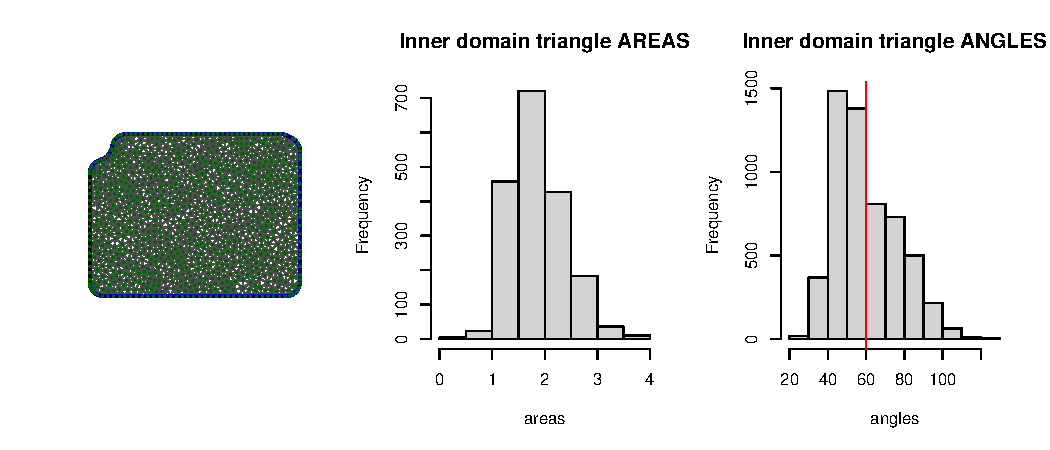
\includegraphics[width=\maxwidth]{figure/checkMesh1-1} 

}


\end{knitrout}
    
This mesh appears to be adequate -- there are not too many large or small triangles and not too many triangles with overly small or large angles. However, in \citet{fos24}, we chose (perhaps unnecessarily) to extend the outer boundary slightly to allow for a better distribution of nodes. This was achieved by adding the argument \texttt{offset=7.5}, which is measured in map units (kilometres in this case). As an example of a `bad' mesh, consider the same spatial region but with fewer nodes.

\begin{knitrout}
\definecolor{shadecolor}{rgb}{0.969, 0.969, 0.969}\color{fgcolor}\begin{kframe}
\begin{alltt}
\hlstd{my.mesh.bad} \hlkwb{<-} \hlkwd{makeMesh}\hlstd{( covars}\hlopt{$}\hlstd{DEM,} \hlkwc{max.n}\hlstd{=}\hlkwd{c}\hlstd{(}\hlnum{250}\hlstd{,} \hlnum{30}\hlstd{),} \hlkwc{dep.range}\hlstd{=}\hlnum{3}\hlstd{,} \hlkwc{doPlot}\hlstd{=}\hlnum{FALSE}\hlstd{)}
\hlkwd{checkMesh}\hlstd{( my.mesh.bad, my.mesh}\hlopt{$}\hlstd{hull,} \hlkwc{ras}\hlstd{=covars}\hlopt{$}\hlstd{DEM)}
\end{alltt}
\end{kframe}

{\centering 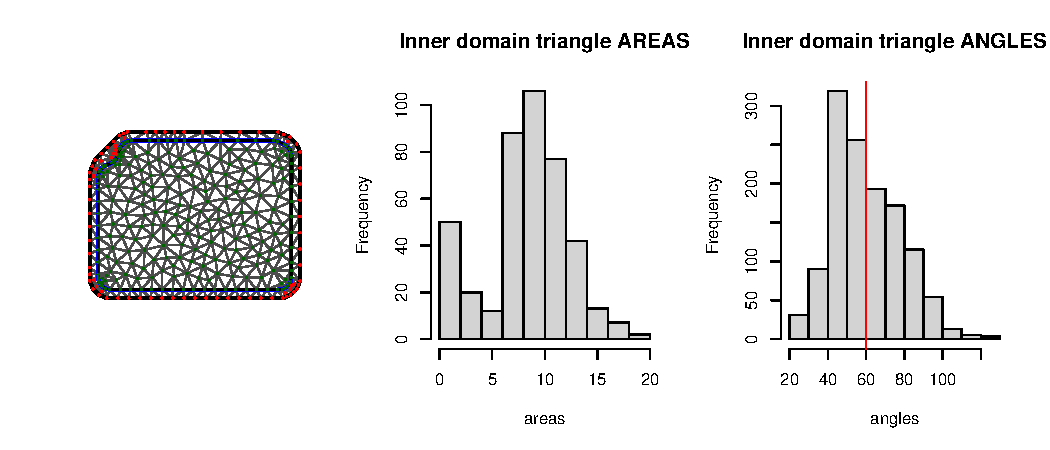
\includegraphics[width=\maxwidth]{figure/makeBadMesh1-1} 

}


\end{knitrout}

The resulting `bad' mesh has mostly good shaped trianlges, but those around the corners of the inner and outer areas are much smaller and more `bunched' than elsewhere. This is picked up in the distribution of the triangle areas, which is quite bimodal. However, the triangle shapes appear to be adequate. In general, the more regular the survey area (non-NA values in the raster layer), the easier it will be to produce an adequate mesh. The survey area for gamba grass is quite regular and hence even this `bad' mesh is not spectacularly bad.
 
\subsection*{Specifying and Evaluating the Model} \label{subsec:mod}

With the data objects and the mesh all curated and created, it is time to (finally) start the formal modelling process. There are, unfortunately, a number of moving parts that need to be specified. Let's go through them in turn.
  
\subsubsection*{Species Distribution}\label{subsubsec:disForm}
  
How the species responds to the environment, as quantified by the layers in the covariate stack (see Section \ref{subsubsec:covs}), is defined through a formula. Terms in this formula apply to \textit{all the different data types}. Specification of this formula parallels almost precisely as one would do for any glm-like modelling process -- see the details section from \texttt{?glm} for more information about forms accepted. This specification allows a wide variety of models to be fitted: linear, curvi-linear (e.g. quadratics), interactions, regression splines, and so on. The formula will take the environmental variables from the covariate stack, and so the terms in the formula must be present there. Currently, the formula will not work with (or at least have unknown, untested behaviour) with factor raster layers -- please be wary when using them and consider expanding them into a set of `dummy' raster layers that indicate the various levels of the factor. 

Like the \texttt{glm} function, the distributionFormula argument can be specified using a saved formula object or a newly specified formula object. It is important to note that, \textit{un}like the \texttt{glm} function, there is no left-hand side to the formula -- there are multiple sources of outcomes and they are hence specified in another argument. Another important aspect of specifying the distribution formula is that \textit{any intercept is stripped out} and to help remind users they are recommended to explicitly add a `0' or a `-1' into the formula. In the ISDM, there are mutliple intercepts and are specified for each data type (at least).

To give some concrete examples about what formulas can be considered in the distribution model, consider these. The last one is the one that is used in \citet{fos24} and is the one that will be continued with here.

\begin{knitrout}
\definecolor{shadecolor}{rgb}{0.969, 0.969, 0.969}\color{fgcolor}\begin{kframe}
\begin{alltt}
\hlcom{#linear in SMRZ only}
\hlstd{my.form} \hlkwb{<-} \hlopt{~}\hlnum{0}\hlopt{+}\hlstd{SMRZ}
\hlcom{#interacting between SMRZ and DEM}
\hlstd{my.form} \hlkwb{<-} \hlopt{~}\hlnum{0}\hlopt{+}\hlstd{SMRZ}\hlopt{*}\hlstd{DEM}
\hlcom{#a B-spline regression basis with low degrees of freedom}
\hlstd{my.form} \hlkwb{<-} \hlopt{~}\hlnum{0}\hlopt{+}\hlstd{splines}\hlopt{::}\hlkwd{bs}\hlstd{(SMRZ,} \hlkwc{df}\hlstd{=}\hlnum{3}\hlstd{)}
\hlcom{#a(n orthogonal) polynomial in SMRZ and DEM}
\hlstd{my.form} \hlkwb{<-} \hlopt{~}\hlnum{0}\hlopt{+}\hlkwd{poly}\hlstd{(SMRZ,}\hlnum{2}\hlstd{)}\hlopt{+}\hlkwd{poly}\hlstd{(DEM,}\hlnum{2}\hlstd{)}
\hlcom{#adding accessibility too (as per paper).}
\hlstd{my.form} \hlkwb{<-} \hlopt{~}\hlnum{0}\hlopt{+}\hlkwd{poly}\hlstd{(SMRZ,}\hlnum{2}\hlstd{)}\hlopt{+}\hlkwd{poly}\hlstd{(DEM,}\hlnum{2}\hlstd{)}\hlopt{+}\hlstd{acc}
\end{alltt}
\end{kframe}
\end{knitrout}

The default action for all covariates in the distribution formula is that they are standardised. This means that they are transformed (linearly -- subtracating mean and deviding by standard deviation), so that the covariate will have zero mean and standard deviation one. This also applies for basis-exansion covariates (like those from \texttt{poly} or {bs}) -- we have found that the scaling for \texttt{poly} is too small. This does not effect the fit of the model but it does improve the numerical stability and has the side effect of altering the scale of the associated model parameter. In turn, this side-effect can make it easier to specify priors for the covariate parameters -- see \ref{subsubsec:priors} for details about how this is done. This behaviour can be `turned off' by using the \texttt{standardiseCovariates} element of the control argument to \texttt{isdm}.
  
One thing that may, at first, seem like an odd omission from the distribution formula is the spatial random effect. This is \textit{never included}. Rather it is included as part of the machinations of \texttt{isdm} (default behaviour) or is not included by explicit request. This is controlled by the \texttt{addRandom} element of the control argument to \texttt{isdm}. 
  
It is difficult to indicate what a `good' and a `bad' distribution formula will look like. It depends solely on the particular species and the covariates that are available. However, analysts should consider elementary pathological cases usually exemplified with linear models. These include avoiding over-fitting. For more basic advice on specification, and some rememdies to common problems please see \citet{net96} or any introductory textbook focussing on linear models.

\subsubsection*{Observation Bias (for PO data)}

The biasFormula argument of \texttt{isdm} specifies how the point pattern that generates the PO data \textit{differs} from the species distribution point pattern. The biasFormula affects \textit{only the PO data} and specifies the model component for the sampling bias for the PO data \citep[see][for example]{war13}. The sampling bias arises from spatially non-uniform sampling effort over the study region. An example of why this might happen is, when PO data is citizen science based, presences are likely to be denser where there are more people available to look for them (ie near population centres). This sampling bias pattern is obscuring the true species distribution and hence should be removed from predictions, if possible. The ISDM allows for this by inspecting the (unbiased) patterns in the PA and AA data, and comparing to the pattern in the PO data.

Specifying the biasFormula argument mirrors that for specifying the distributionFormula argument. It is any formula object which takes data from the raster stack. It is limited by the same limitations and transformations as the distributionFormula (see Section \ref{subsubsec:disForm}). However, note that an intercept is needed -- it is the intercept for the PO point process. If removed, in the biasFormula argument, then \texttt{isdm} will assume that it is intended and not fit an intercept. An intercept is included by default, just like \texttt{glm}.

The biasFormula argument should contain terms that are likely to affect the anathropegenic search pattern. Often these will include variables like `travel time to location' and `search intensity of other species'. However, specifics will depend on the data available and the particular system being modelled.

In the gamba grass example, \citet{fos24} used a simple structure based on accessibility. There is no estimability issue with including the term in both the biasFormula and in the distributionFormula -- the latter is based on both PO and PA/AA data, while the former is based only on the PO data. However, in the particular case when there is only PO data, then the same covariate should not be included in both formulas.

Here are some examples of bias formulas for the gamba grass example. We take the last, simple formula to progress with.
\begin{knitrout}
\definecolor{shadecolor}{rgb}{0.969, 0.969, 0.969}\color{fgcolor}\begin{kframe}
\begin{alltt}
\hlcom{#intercept only == no heterogeneity in search effort}
\hlstd{my.biasForm} \hlkwb{<-} \hlnum{1}
\hlcom{#regression spline in acc}
\hlstd{my.biasForm} \hlkwb{<-} \hlopt{~}\hlnum{1}\hlopt{+}\hlstd{splines}\hlopt{::}\hlkwd{bs}\hlstd{( acc,} \hlkwc{df}\hlstd{=}\hlnum{3}\hlstd{)}
\hlcom{#linear in acc}
\hlstd{my.biasForm} \hlkwb{<-} \hlopt{~}\hlnum{1}\hlopt{+}\hlstd{acc}
\end{alltt}
\end{kframe}
\end{knitrout}

\subsubsection*{Sampling Artefacts (for AA and PA data)}

The PA and AA data may contain sources of variation that are not a result of species distribution. This is in spite of the assumption that the PA and AA data are the result of a well-planned survey effort. Such variation may arise from (but not limited to): 1) different measurement tools/procedures, 2) blocking or stratification, or 3) seasons or weather. In fact, any source of variation that may cause extraneous variation in the data can be modelled here. We call these sources of variation \textit{sampling artefacts} as they are due to the sampling process and are generally not of primary interest.

There should be a sampling artefact formula for each of the data types included in the model. However, the PO sampling artefact is nonsensical and is ignored. Sampling artefacts \textit{only affect those data types that they are defined for} and are in addition to the distribution formula for these observations. The formulae follow the same general rules as all formulas except that we currently \textit{do not} recommend the use of basis expansion within the formula itself. If the user wants to use basis expansion, then they should create a temporary design matrix object, that includes the basis expanded variables, prior to calling \texttt{isdm} and use those names instead. Of course, there are exceptions to this rule, but they have not been tested and hence it is safer just to follow the pre-expansion principle.

Once again, there is no restriction about what varaibles are included in the artefactFormulas. Variables can appear in here that also appear in the distributionFormula (for example). However, the user must seriously ask themselves `why'? Why would the variation within the PA/AA data be dependent on that variable \textit{after the distribution has been conditioned out}?
    
For the gamba grass example, there is only one source of PA data (and no AA data). The PA data all come from a single data source, which were all measured using the same sampling tool (an aerial survey). For this reason, it is likely to be reasonable to assume that there are no sampling artefacts within these PA data. This is the assumption made in \citet{fos24} and is the assumption that we move forward with. However, the data also contain the observer that took the measurement. Different observers may see/perceive/report differently and so we present their inclusion an (untested) alternative for instructional purposes.
\begin{knitrout}
\definecolor{shadecolor}{rgb}{0.969, 0.969, 0.969}\color{fgcolor}\begin{kframe}
\begin{alltt}
\hlcom{#observer differences as a sampling artefact}
\hlkwd{list}\hlstd{(} \hlkwc{PA}\hlstd{=}\hlopt{~}\hlnum{1}\hlopt{+}\hlstd{observer)}
\end{alltt}
\begin{verbatim}
$PA
~1 + observer
\end{verbatim}
\begin{alltt}
\hlcom{#intercept only == no sampling artefact }
\hlcom{#               == no heterogeneity within each data type}
\hlkwd{list}\hlstd{(} \hlkwc{PA}\hlstd{=}\hlopt{~}\hlnum{1}\hlstd{)}
\end{alltt}
\begin{verbatim}
$PA
~1
\end{verbatim}
\end{kframe}
\end{knitrout}
    
\subsubsection*{Bringing it All Together: an initial model estimation}
  
We now have enough pieces to estimate the model. This will rely on default parameters, which could be dangerous in some situations. Nevertheless, this is done to demonstrate the mechanics of the estimation. It is stressed that this is a preliminary model estimate -- wihtout due consideration to priors (especially those of the spatial random effect) the results may be `odd'. Even though it is not explicitly stated, this model contains a spatial random effect in the distribution formula. This term is considered fundamental enough, that it has to be explicitly removed (instructions later).

The components that make up this model estimate have nearly all been introduced before. The exceptions are those that specify which variable should be used for what in which data set. That was a confusing sentence, so we'll break it down.
  
The responseNames argument lists what variables should be used for outcomes for each of the data types. It is a text label. Here, it specifies that the variable ``PA'' should be used from the data.frame \texttt{gamba\_PA}, which is specified in observationList\$PAdat.
  
The sampleAreaNames argument informs which variable within each of the PA and AA data.frames give the sample area. As stated before the sample area is the area that the sampling covered. For the gamba PA data, the sampling area was constant, and held in the un-creatively named variable ``Area''. There is no requirement for the PO data to have an area associated with it (these are assumed to be a point).
  
Finally, \texttt{isdm} must be told what the coordinates are called. These must be the same for all data structures. It is specified through the control\$coord.names argument.
  
\begin{knitrout}
\definecolor{shadecolor}{rgb}{0.969, 0.969, 0.969}\color{fgcolor}\begin{kframe}
\begin{alltt}
\hlstd{fm} \hlkwb{<-} \hlkwd{isdm}\hlstd{(} \hlkwc{observationList}\hlstd{=}\hlkwd{list}\hlstd{(} \hlkwc{POdat}\hlstd{=gamba_PO,}
                                  \hlkwc{PAdat}\hlstd{=gamba_PA),}
            \hlkwc{covars}\hlstd{=covars,}
            \hlkwc{mesh}\hlstd{=my.mesh,}
            \hlkwc{responseNames}\hlstd{=}\hlkwd{c}\hlstd{(} \hlkwc{PO}\hlstd{=}\hlkwa{NULL}\hlstd{,} \hlkwc{PA}\hlstd{=}\hlstr{"PA"}\hlstd{),}
            \hlkwc{sampleAreaNames}\hlstd{=}\hlkwd{c}\hlstd{(} \hlkwc{PO}\hlstd{=}\hlkwa{NULL}\hlstd{,} \hlkwc{PA}\hlstd{=}\hlstr{"Area"}\hlstd{),}
            \hlkwc{distributionFormula}\hlstd{=}\hlopt{~}\hlnum{0}\hlopt{+}\hlkwd{poly}\hlstd{( DEM,} \hlnum{2}\hlstd{)} \hlopt{+} \hlkwd{poly}\hlstd{( SMRZ,}\hlnum{2}\hlstd{)} \hlopt{+} \hlstd{ACC,}
            \hlkwc{biasFormula}\hlstd{=}\hlopt{~}\hlnum{1}\hlopt{+}\hlstd{ACC,}
            \hlkwc{artefactFormulas}\hlstd{=}\hlkwd{list}\hlstd{(} \hlkwc{PA}\hlstd{=}\hlopt{~}\hlnum{1}\hlstd{),}
            \hlkwc{control}\hlstd{=}\hlkwd{list}\hlstd{(} \hlkwc{coord.names}\hlstd{=}\hlkwd{c}\hlstd{(}\hlstr{"x"}\hlstd{,}\hlstr{"y"}\hlstd{)))}
\end{alltt}
\end{kframe}
\end{knitrout}
    
The return from \texttt{isdm} is silent, so there is nothing special to see upon its successful completion. Given this initial fit, further refinements of the model can be demonstrated.
  
\subsubsection*{Priors for Model Effects} \label{subsubsec:priors}
  
All Bayesian analyses require the user to specify a prior distribution, and this ISDM is no different. In \texttt{RISDM}, we have focussed on ease of specification rather than full flexibility. We focus on specifying vague priors and separate only priors for intercepts and priors for covariate effects. We envisage that most users will specify models with vague priors, reflecting little or now prior knowledge, which fits easily into this format.
  
The priors are specified via the control list argument and describe Gaussian distributions. In particular, the priors are specified through the prior.mean element and the prior.sd (or prior.prec) arguments. The prior.mean is a single scalar giving the prior expectation of \textit{all} the model's effects. This includes all intercepts and all covariate effects for all the data types. Almost always, prior.mean will be zero, indicating that the effect has a priori equal chance of being positive or negative.

The prior variation for the covariate effects are split into two types: those for intercepts and those for covariate effects. We prefer to specify prior variation through standard deviation, but also allow for precision to be specified (inversely related). These variances are specified through the \texttt{int.sd} and \texttt{int.prec} elements of the control list. By default the sd for the intercepts is very large (1000) and that for the covariate effects is large (10). We note that if a standard deviation is specified then the precision is ignored.

Remember, from Section \ref{subsubsec:disForm} that all covariates are scaled prior to fitting the model. This means that the effects are \textit{in some sense} on the same numerical scale. In turn this implies that it may be justifiable, or at least practical, to specify this common prior for effects. If a particular application requires a different approach then the priors will have to be specified directly.

If the user wants to specify priors directly, then they can by specifying prior.list element of the control list directly. This argument is \textit{passed directly} to the INLA call, and so the specification is solely the responsibility of the user. INLA requires that these are passed as a list of two named elements: mean and prec. Each element contains the named vector of values for the prior. Note that only those effects that are desired to be \textit{different} from the default are required to be named and specified (I think).

Here are some control list examples that specifies various prior formulations. Note that these specify only those control elements for the priors; other terms may be added to this list to control other aspects of the model or the computational aspects.
\begin{knitrout}
\definecolor{shadecolor}{rgb}{0.969, 0.969, 0.969}\color{fgcolor}\begin{kframe}
\begin{alltt}
\hlcom{#the very vague everything}
\hlstd{my.control} \hlkwb{<-} \hlkwd{list}\hlstd{(} \hlkwc{prior.mean}\hlstd{=}\hlnum{0}\hlstd{,} \hlkwc{int.sd}\hlstd{=}\hlnum{1000}\hlstd{,} \hlkwc{other.sd}\hlstd{=}\hlnum{1000}\hlstd{)}
\hlcom{#(much) tighter prior for effects}
\hlstd{my.control} \hlkwb{<-} \hlkwd{list}\hlstd{(} \hlkwc{prior.mean}\hlstd{=}\hlnum{0}\hlstd{,} \hlkwc{int.sd}\hlstd{=}\hlnum{1000}\hlstd{,} \hlkwc{other.sd}\hlstd{=}\hlnum{0.1}\hlstd{)}
\hlcom{#the default}
\hlstd{my.control} \hlkwb{<-} \hlkwd{list}\hlstd{(} \hlkwc{prior.mean}\hlstd{=}\hlnum{0}\hlstd{,} \hlkwc{int.sd}\hlstd{=}\hlnum{1000}\hlstd{,} \hlkwc{other.sd}\hlstd{=}\hlnum{10}\hlstd{)}
\end{alltt}
\end{kframe}
\end{knitrout}

\subsubsection*{Spatial Effects via SPDE}

The \texttt{RISDM} model, by default, includes a spatial random effect. This spatial effect is defined according to the SPDE approach defined in \citet{lin11} and practical aspects discussed in \citet{lin15} and is included for 2 purposes: 1) to induce a spatial autocorrelation into the observations (the random effect is spatially correlated); and 2) to explain spatially patterned random variation (noise) that has not been explained by the environmental covariates.

The specification of the distribution of the random effects depends on two parameters: the standard deviation of the effects, and the spatial range of their dependence. The spatial range is approximately the distance that samples must be separated by before data from those locations are expected to be almost independent (correlation of approximately 0.1). Both these parameters require a prior distribution to be specified, and \texttt{RISDM}, like \texttt{INLA}, follows \citet{sim17} by using complexity priors. These priors are defined by defining the prior chance that the parameter falls above (for prior standard deviation) or below (for spatial range) specified values. For the gamba grass example, it may be reasonable that the standard deviation has probability of 0.1 (10\% chance) of being above 5. We feel that this is a vague prior for random effects on a log-link scale. Likewise, a vague prior for spatial dependence could be that there is a probability of 0.1 that the range is less than 1km. The previous initial model can be updated using these priors, giving the model in \citet{fos24}.

\begin{knitrout}
\definecolor{shadecolor}{rgb}{0.969, 0.969, 0.969}\color{fgcolor}\begin{kframe}
\begin{alltt}
\hlstd{fm} \hlkwb{<-} \hlkwd{isdm}\hlstd{(} \hlkwc{observationList}\hlstd{=}\hlkwd{list}\hlstd{(} \hlkwc{POdat}\hlstd{=gamba_PO,}
                                  \hlkwc{PAdat}\hlstd{=gamba_PA),}
            \hlkwc{covars}\hlstd{=covars,}
            \hlkwc{mesh}\hlstd{=my.mesh,}
            \hlkwc{responseNames}\hlstd{=}\hlkwd{c}\hlstd{(} \hlkwc{PO}\hlstd{=}\hlkwa{NULL}\hlstd{,} \hlkwc{PA}\hlstd{=}\hlstr{"PA"}\hlstd{),}
            \hlkwc{sampleAreaNames}\hlstd{=}\hlkwd{c}\hlstd{(} \hlkwc{PO}\hlstd{=}\hlkwa{NULL}\hlstd{,} \hlkwc{PA}\hlstd{=}\hlstr{"Area"}\hlstd{),}
            \hlkwc{distributionFormula}\hlstd{=}\hlopt{~}\hlnum{0}\hlopt{+}\hlkwd{poly}\hlstd{( DEM,} \hlnum{2}\hlstd{)} \hlopt{+} \hlkwd{poly}\hlstd{( SMRZ,}\hlnum{2}\hlstd{)} \hlopt{+} \hlstd{ACC,}
            \hlkwc{biasFormula}\hlstd{=}\hlopt{~}\hlnum{1}\hlopt{+}\hlstd{ACC,}
            \hlkwc{artefactFormulas}\hlstd{=}\hlkwd{list}\hlstd{(} \hlkwc{PA}\hlstd{=}\hlopt{~}\hlnum{1}\hlstd{),}
            \hlkwc{control}\hlstd{=}\hlkwd{list}\hlstd{(} \hlkwc{coord.names}\hlstd{=}\hlkwd{c}\hlstd{(}\hlstr{"x"}\hlstd{,}\hlstr{"y"}\hlstd{),}
                          \hlkwc{int.sd}\hlstd{=}\hlnum{1000}\hlstd{,} \hlkwc{other.sd}\hlstd{=}\hlnum{10}\hlstd{,} \hlkwc{prior.mean}\hlstd{=}\hlnum{0}\hlstd{,}
                          \hlkwc{prior.range}\hlstd{=}\hlkwd{c}\hlstd{(}\hlnum{1}\hlstd{,}\hlnum{0.1}\hlstd{),} \hlkwc{prior.space.sigma}\hlstd{=}\hlkwd{c}\hlstd{(} \hlnum{5}\hlstd{,}\hlnum{0.1}\hlstd{)))}
\end{alltt}
\end{kframe}
\end{knitrout}

The addition of the spatial random effect can be suppressed by the control list element. That is by including addRandom=FALSE into the control=list($\ldots$) argument. Code below. The model will be much (!) faster to estimate.  We'll return to this model later in the vignette.
  
\begin{knitrout}
\definecolor{shadecolor}{rgb}{0.969, 0.969, 0.969}\color{fgcolor}\begin{kframe}
\begin{alltt}
\hlstd{fm.noRand} \hlkwb{<-} \hlkwd{isdm}\hlstd{(} \hlkwc{observationList}\hlstd{=}\hlkwd{list}\hlstd{(} \hlkwc{POdat}\hlstd{=gamba_PO,}
                                         \hlkwc{PAdat}\hlstd{=gamba_PA),}
                   \hlkwc{covars}\hlstd{=covars,}
                   \hlkwc{mesh}\hlstd{=my.mesh,}
                   \hlkwc{responseNames}\hlstd{=}\hlkwd{c}\hlstd{(} \hlkwc{PO}\hlstd{=}\hlkwa{NULL}\hlstd{,} \hlkwc{PA}\hlstd{=}\hlstr{"PA"}\hlstd{),}
                   \hlkwc{sampleAreaNames}\hlstd{=}\hlkwd{c}\hlstd{(} \hlkwc{PO}\hlstd{=}\hlkwa{NULL}\hlstd{,} \hlkwc{PA}\hlstd{=}\hlstr{"Area"}\hlstd{),}
                   \hlkwc{distributionFormula}\hlstd{=}\hlopt{~}\hlnum{0}\hlopt{+}\hlkwd{poly}\hlstd{( DEM,} \hlnum{2}\hlstd{)} \hlopt{+} \hlkwd{poly}\hlstd{( SMRZ,}\hlnum{2}\hlstd{)} \hlopt{+} \hlstd{ACC,}
                   \hlkwc{biasFormula}\hlstd{=}\hlopt{~}\hlnum{1}\hlopt{+}\hlstd{ACC,}
                   \hlkwc{artefactFormulas}\hlstd{=}\hlkwd{list}\hlstd{(} \hlkwc{PA}\hlstd{=}\hlopt{~}\hlnum{1}\hlstd{),}
                   \hlkwc{control}\hlstd{=}\hlkwd{list}\hlstd{(} \hlkwc{coord.names}\hlstd{=}\hlkwd{c}\hlstd{(}\hlstr{"x"}\hlstd{,}\hlstr{"y"}\hlstd{),}
                                  \hlkwc{int.sd}\hlstd{=}\hlnum{1000}\hlstd{,} \hlkwc{other.sd}\hlstd{=}\hlnum{10}\hlstd{,} \hlkwc{prior.mean}\hlstd{=}\hlnum{0}\hlstd{,}
                                  \hlkwc{addRandom}\hlstd{=}\hlnum{FALSE}\hlstd{))}
\end{alltt}
\end{kframe}
\end{knitrout}
    
\subsection*{Diagnostics and Summary}
  
To understand how the model has performed, and to check that things have gone as could reasonably be expected, it is important to both check the model for obvious (large) departures from assumptions and to check if the estimated model passes a `laugh test'. Both these checks have been performed in statstical sciences for a long time, but perhaps only the diagnostic formed by checking for departures is formally defined anywhere. Tools for both approaches will be given now.

\subsubsection*{Summary Tables} \label{subsubsec:summ}

To obtain an elementary understanding of the estimated model, a \texttt{summary} method is provided. This, like the method for \texttt{glm}, gives information about the estimated parameters and a statistic about the model itself. Unlike a \texttt{glm} summary method, the \texttt{isdm} summary method will not print the model call itself as it is generally quite long, cryptic and boring. If users want to see the \texttt{INLA} call then they can, as part of the return object (fm\$mod\$call in this case).

The printed summary object shows univariate summaries of the modelled parameters' posterior distributions. These are arranged into the type of effect (distribution, bias, artefact) for ease of interpretation. In this case, we see that both quadratic terms in the distribution formula poly.DEM.2.2 and poly.SMRZ.2.2 are negative and with credible intervals that do not cover zero. This implies that both relationships are concave in shape, over the observed covariate ranges. This is reassuring as it aggrees somewhat with niche theory, but it is not the final word (linear effect may still outweigh the quadratic). The accessibility covariate is strongly negative, implying that those locations that are remote (high accessibility values) are less likely to have gamba grass. The other model components can be likewise interpreted.
  
\begin{knitrout}
\definecolor{shadecolor}{rgb}{0.969, 0.969, 0.969}\color{fgcolor}\begin{kframe}
\begin{alltt}
\hlkwd{summary}\hlstd{( fm)}
\end{alltt}
\begin{verbatim}
$DISTRIBUTION
                     mean         sd    0.025quant    0.5quant 0.975quant
poly.DEM.2.1   0.23898279 0.12155317 -0.0008501594  0.23948557  0.4759722
poly.DEM.2.2  -0.39567315 0.08560623 -0.5635820572 -0.39567217 -0.2277701
poly.SMRZ.2.1  0.03762871 0.24846410 -0.4561825083  0.03957789  0.5204453
poly.SMRZ.2.2 -0.56086587 0.20891208 -0.9757263351 -0.55928330 -0.1549695
ACC           -1.93507665 0.20521489 -2.3398860438 -1.93425929 -1.5348902

$PO_BIAS
                  mean        sd 0.025quant  0.5quant 0.975quant
PO_Intercept -3.378855 0.2483792  -3.894271 -3.369569 -2.9173456
PO_ACC       -1.141882 0.1378065  -1.412156 -1.141877 -0.8716359

$PA_ARTEFACT
                  mean        sd 0.025quant  0.5quant 0.975quant
PA_Intercept -14.09951 0.2767023   -14.6647 -14.09211  -13.57715

$SPATIAL
                            mean         sd 0.025quant 0.5quant 0.975quant
Range for isdm.spat.XXX 3.050350 0.37128116   2.417175 3.015973   3.876087
Stdev for isdm.spat.XXX 2.269715 0.09543608   2.086649 2.267875   2.463519

$marg.lik
[1] -3868.7

attr(,"class")
[1] "summary.isdm"
\end{verbatim}
\end{kframe}
\end{knitrout}
    
\subsubsection*{Model Comparison}

The \texttt{summary.isdm} method returns, as a member of the list, an INLA estimate of the marginal likelihood. This is sometimes referred to as `model evidence'. It can be used to compare models, in particular using Bayes Factors. For further information, the reader is referred to \citet{kas95} but also see \citet{gel13}.
    
\subsubsection*{Residual Plots} \label{subsubsec:res}
  
Residuals give an analyst a view of the data through the lens of the model. As such, they can help identify inadequacies from tenuous model assumptions. Residuals \textit{can} even help identify possible remedies to inadequacies \citep[e.g.][]{net96}.
  
In linear models (e.g. multiple linear regressions) residuals have a natural definition -- the observation minus the model prediction. This works in that case because those deviations are assumed by the model to be normally distributed (and homoscedastic) and there are no random effects, apart from residuals, in the model. In general use, residuals do not incorporate the variability in the model prediction. In a full Bayesian treatment, this extra variability would be included.
  
In \texttt{RISDM}, randomised quantile residuals \citep[RQR;][]{dun96} are used. These residuals have a number of desireable features. Most notably, their distribution (assuming model assumptions are correct) is known, and is common for all different data types. This is in contrast to, say, Pearson or deviance residuals whose distribution is unknown for a finite sample \citep{dun96}. The RQR residuals incorporate only the variation from the final fitted value (including the spatial random effect) to the observation. This mirrors the residual treatment in the popular \texttt{mgcv} package \citep{woo17}, even if \texttt{mgcv} uses different types of residuals. If the model is adequately specified, then the RQR should be normally distributed and homoscedastic -- like residuals from a multiple linear regression. Departures from normality, or patterns along environmental gradients or through space may indicate problems with the model.
  
In \texttt{RISDM} there are multiple sets of residuals -- one for each data type. All these residuals can be calculated using the \texttt{residuals.isdm} method. Most often, the user will want to plot these residuals and this can be done in an automated way using the \texttt{plot.isdm} method, in ways that may be useful for diagnosing inadequacies. These mirror the treatment in introductory textbooks on linear models \citep[e.g.][]{net96}. Resdiuals are plotted per data type using a residuals versus fitted and a quantile-quantile (Q-Q) plot. There should be no patterning in the residuals versus fitted plot, in either mean pattern or in residual variation. The following plot for PA residuals shows no cause for concern here, and the PO residuals are harder to interpret. The Q-Q plot should follow a straight line. The following plot seems fine for PA data, but questionable for PO data. \texttt{RISDM} will also plot the PO RQR residuals as a spatial layer. Like any covariate, there should be no patterning and its presence could indicate deficiencies.
  
\begin{knitrout}
\definecolor{shadecolor}{rgb}{0.969, 0.969, 0.969}\color{fgcolor}\begin{kframe}
\begin{alltt}
\hlkwd{plot}\hlstd{( fm,} \hlkwc{covars}\hlstd{=covars,} \hlkwc{nFigRow}\hlstd{=}\hlnum{2}\hlstd{,} \hlkwc{ask}\hlstd{=}\hlnum{FALSE}\hlstd{)}
\end{alltt}
\end{kframe}\begin{figure}

{\centering 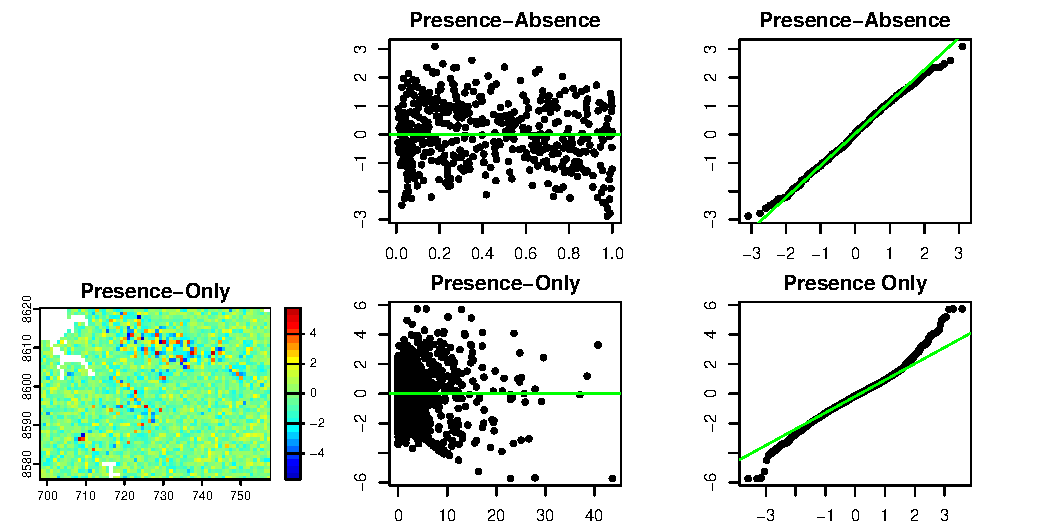
\includegraphics[width=\maxwidth]{figure/residPlots-1} 

}

\caption[Residual plots for the gamba grass data, and the model containing quadratic effects and a spatial term]{Residual plots for the gamba grass data, and the model containing quadratic effects and a spatial term.}\label{fig:residPlots}
\end{figure}

\end{knitrout}
    
One open research questions around residuals is trying to determine how large the departures need to be before the model needs altering. This will depend on many different aspects, including the type of inference sought. Hence, it is not clear if the residuals in Figure \ref{fig:residPlots} indicate an adequate model or not. However, it is possible (and easy) to demonstrate a model with \textit{a worse fit}. To do this, we revisit the model but exclude the spatial random effects. The resulting residual plots are in Figure \ref{fig:residPlots2}. The PA data still seem adequately represented but the patterns in the PO data are accentuated and are now obviously worrisome. There are strong spatial patterns and the residuals are obviously non-normal.
  
\begin{knitrout}
\definecolor{shadecolor}{rgb}{0.969, 0.969, 0.969}\color{fgcolor}\begin{kframe}
\begin{alltt}
\hlkwd{plot}\hlstd{( fm.noRand,} \hlkwc{covars}\hlstd{=covars,} \hlkwc{nFigRow}\hlstd{=}\hlnum{2}\hlstd{,} \hlkwc{ask}\hlstd{=}\hlnum{FALSE}\hlstd{)}
\end{alltt}
\end{kframe}\begin{figure}

{\centering 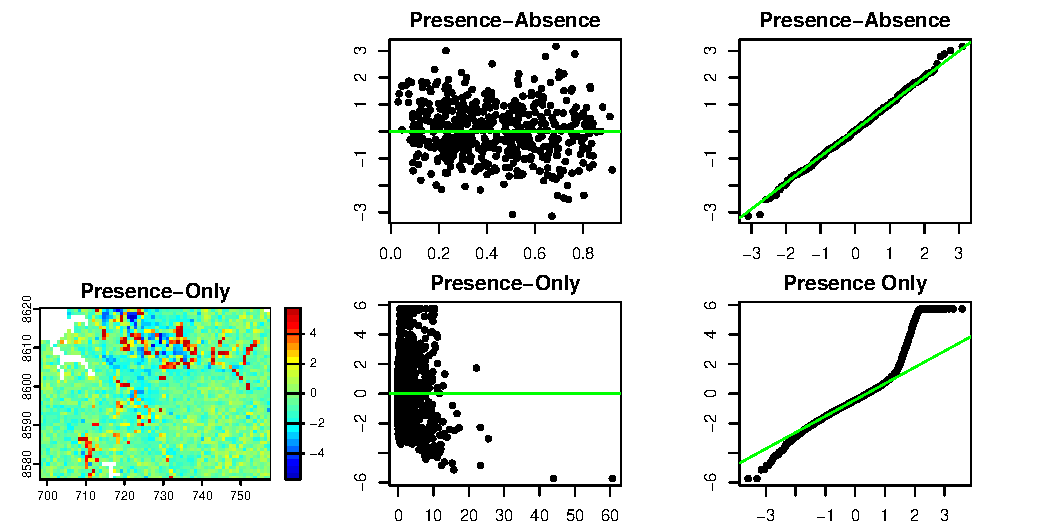
\includegraphics[width=\maxwidth]{figure/residPlots2-1} 

}

\caption[Residual plots for the gamba grass data, and the model containing quadratic effects 	extit{but no spatial term}]{Residual plots for the gamba grass data, and the model containing quadratic effects 	extit{but no spatial term}.}\label{fig:residPlots2}
\end{figure}

\end{knitrout}
    
One of the potential short-comings of RQR residuals is that they contain a random component. This component is largest for data types that have few categories dichotomous data, like PA data, are subject to the largest amount possible. This fact may contribute to the apparent adequate residual plots for the model without spatial random effects.
  
\subsection*{Prediction} \label{subsec:pred}
  
Predictions from the fitted model are performed using the \texttt{predict.isdm} method. This method proceeds by taking posterior draws of the parameters, using \texttt{INLA}'s \texttt{inla.posterior.sample} function, and then predicting using the sampled parameters into a user-supplied raster stack. In this routine, the spatial random effects are treated the same as the parameters. This is demonstrated using both the model with (and without) spatial random effects.

One choice that the user should make is which intercept should be included in the model. This choice has a real consequence in the predictions as some datasets (or even data types) will naturally have higher/lower intercepts due to tool efficacy and possibly just by measuring the geographical area that it did.

By default the \texttt{predict} method will predict on the intensity scale. This gives the expected number of individuals within a raster cell at each of the raster's locations. However, this is not the only choice and the user can choose to predict the probability of presence or the linear predictor. Probability is a non-linear transformation of the intensity and, as such, is dependent upon the intercept value chosen. An intercept that is abnormally high will produce values that are too close to one. Likewise, an intercept that is low will have deflated probability. Care should be taken and the choice should be reasoned and well-considered.

The intensity and probability predictions in Figure \ref{fig:pred} appear to be very similar. They are. This is because the intensity and probability are very small, and when they are very small the non-linear transformation between them turns out to be very well approximated by the identity function.
  
The \texttt{predict} method outputs a list with a number of elements. Arguably, the most useful of these is the `field' element, which contains a raster stack with a number of summaries of the prediction posterior. Most notably, the prediction stack contains the median prediction and the 2.5\% percentile and the 97.5\% percentile. These values can be taken to be the point and the interval estimate for the predicted property. Also included in the prediction stack is the posterior mean and the posterior standard deviation. It has been the authors experience that the median is a more robust summary of central location in this situation, and it is recommended.
  
\begin{knitrout}
\definecolor{shadecolor}{rgb}{0.969, 0.969, 0.969}\color{fgcolor}\begin{kframe}
\begin{alltt}
\hlcom{#You should use a much(!) larger value of S.}
\hlcom{#You may want to choose a larger value of n.threads too.}
\hlstd{fm}\hlopt{$}\hlstd{preds} \hlkwb{<-} \hlkwd{predict}\hlstd{( fm,} \hlkwc{covars}\hlstd{=covars,} \hlkwc{S}\hlstd{=}\hlnum{50}\hlstd{,}
                       \hlkwc{intercept.terms}\hlstd{=}\hlstr{"PA_Intercept"}\hlstd{)}
\hlkwd{plot}\hlstd{( fm}\hlopt{$}\hlstd{preds}\hlopt{$}\hlstd{field)}

\hlcom{#Predicting probability too}
\hlstd{fm}\hlopt{$}\hlstd{preds.probs} \hlkwb{<-} \hlkwd{predict}\hlstd{( fm,} \hlkwc{covars}\hlstd{=covars,}
                           \hlkwc{S}\hlstd{=}\hlnum{50}\hlstd{,} \hlkwc{intercept.terms}\hlstd{=}\hlstr{"PA_Intercept"}\hlstd{,}
                           \hlkwc{type}\hlstd{=}\hlstr{"probability"}\hlstd{)}
\hlkwd{plot}\hlstd{( fm}\hlopt{$}\hlstd{preds.probs}\hlopt{$}\hlstd{field)}
\end{alltt}
\end{kframe}\begin{figure}

{\centering 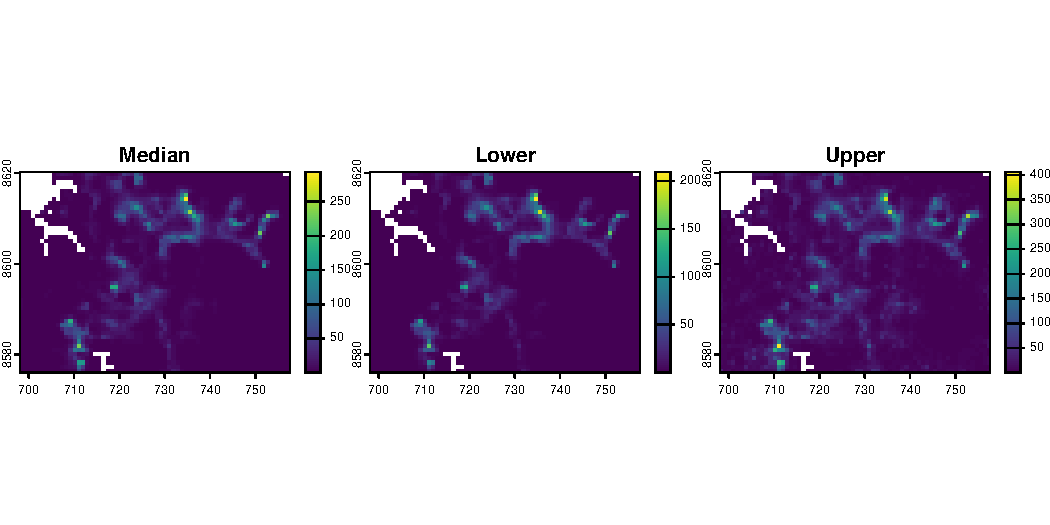
\includegraphics[width=\maxwidth]{figure/pred-1} 
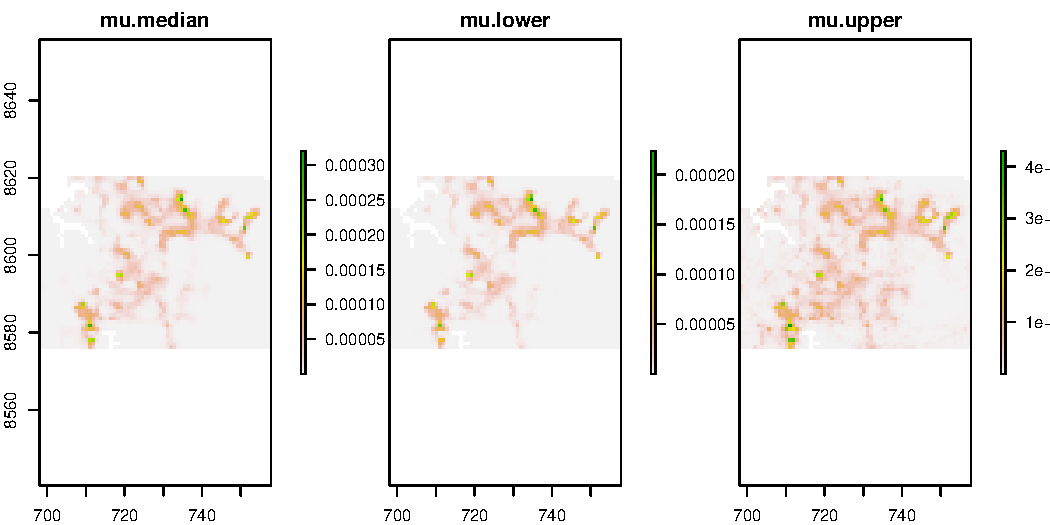
\includegraphics[width=\maxwidth]{figure/pred-2} 

}

\caption[Predictions from the quadratic model including random effects]{Predictions from the quadratic model including random effects. Upper two rows are for the intensity, and bottom two rows are predictions of the probability of presence (within a raster cell)}\label{fig:pred}
\end{figure}

\end{knitrout}
    
By default, the \texttt{predict.isdm} method includes the terms from the distribution function (including spatial random effect) and whatever intercept is chosen. However, variations on this can be achieved:
\begin{itemize}
  \item The inclusion of the random effect can be switched on and off by using the `includeRandom' argument. 
  \item The inclusion of the fixed effect component of the linear predictor can be switched on/off by using the `includeFixed=FALSE' argument.
  \item The terms in the sampling bias model component (not included by default) can be included or not using the `includeBias' argument.
\end{itemize}
Combinations of these three arguments will give the user any combination of effect types that they want. This option is included to inspect the relative contribution from the terms, for understanding, education and possibly diagnosis. As yet, it is unclear if there is any inferential use.
    
\subsection*{Interpretation} \label{subsec:inter}

Interpretation of any non-experimental (e.g. survey and unplanned) data requires care. This is because the inferences may change depending on what assumptions the analyst makes, and what data (covariates) are available. Just one example: if a key covariate is not measured, or is measured with high variance, then the effect of that covariate may be erroneously partitioned to other sources. Nevertheless, in the hope (and assumption) that these types of scenarios are the minority, it can be useful to try and understand how the model is working. Our opinion is that these procedures should be considered as `hypothesis generating' rather than hard evidence for any particular theory. The reason is that there could be multiple pathways to the result. Just one of the probably less-interesting pathways is that the result depends just on random chance in the data.

Interpreting the model involves inspecting the posterior distribution of the model's parameters. When the terms are linear, this is pretty simple to do.  However, when there is some sort of basis expansion in the formula (e.g. quadratic or B-spline) then it becomes more difficult. One solution (not used here) is to pre-compute all basis expansions before fitting the model. The responses can then be constructed using the posterior distributions. Another option is to let \texttt{predict.isdm} do the work -- we will use this now. Note that the data, for the covariate of interest, must be exactly the same as the data used in the model estimation. If this is not the case, then there will be a different basis expansion envoked which will create a different relationship (not the one modelled).

The covariate effects for gamba grass are presented in Figure \ref{fig:interp}. Note that there is a bit of coding involved; there is no function within \texttt{RISDM} to do this directly and the predict function must be `appropriately tricked'. Besides plotting nearly always takes some extra lines of code. Whilst details are important, the process is actually fairly straight-forward: 1) create a raster layer with a constant value for the habitatArea offset, 2) predict specifying which terms should be included, and 3) plot)

\begin{knitrout}
\definecolor{shadecolor}{rgb}{0.969, 0.969, 0.969}\color{fgcolor}\begin{kframe}
\begin{alltt}
\hlcom{#the data for interpretation}
\hlcom{#adding a temporary cell area layer}
\hlstd{covarsForInter} \hlkwb{<-} \hlkwd{addLayer}\hlstd{( covars, covars[[}\hlnum{1}\hlstd{]])}
\hlkwd{names}\hlstd{( covarsForInter)} \hlkwb{<-} \hlkwd{c}\hlstd{(} \hlkwd{names}\hlstd{( covars),} \hlstr{"tmp.habiArea"}\hlstd{)}
\hlcom{#area is now constant with log(1)=0 contribution}
\hlkwd{values}\hlstd{( covarsForInter}\hlopt{$}\hlstd{tmp.habiArea)} \hlkwb{<-} \hlnum{1}

\hlcom{#You could use a much(!) larger value of S.}
\hlstd{interpPreds} \hlkwb{<-} \hlkwd{predict}\hlstd{( fm,} \hlkwc{covars}\hlstd{=covarsForInter,}
                        \hlkwc{habitatArea}\hlstd{=}\hlstr{"tmp.habiArea"}\hlstd{,} \hlkwc{S}\hlstd{=}\hlnum{50}\hlstd{,}
                        \hlkwc{includeFixed}\hlstd{=}\hlstr{"SMRZ"}\hlstd{,} \hlkwc{includeRandom}\hlstd{=}\hlnum{FALSE}\hlstd{,} \hlkwc{type}\hlstd{=}\hlstr{"link"}\hlstd{)}

\hlcom{#compile covariate and prediction}
\hlstd{pred.df} \hlkwb{<-} \hlkwd{as.data.frame}\hlstd{(} \hlkwd{cbind}\hlstd{(} \hlkwc{SMRZ}\hlstd{=}\hlkwd{values}\hlstd{( covars}\hlopt{$}\hlstd{SMRZ),}
     \hlkwd{values}\hlstd{( interpPreds}\hlopt{$}\hlstd{field[[}\hlkwd{c}\hlstd{(}\hlstr{"mu.median"}\hlstd{,}\hlstr{"mu.lower"}\hlstd{,}\hlstr{"mu.upper"}\hlstd{)]])))}
\hlcom{#plot}
\hlstd{pred.df} \hlkwb{<-} \hlstd{pred.df[}\hlopt{!}\hlkwd{is.na}\hlstd{( pred.df}\hlopt{$}\hlstd{SMRZ),]}
\hlstd{pred.df} \hlkwb{<-} \hlstd{pred.df[}\hlkwd{order}\hlstd{( pred.df}\hlopt{$}\hlstd{SMRZ),]}
\hlkwd{matplot}\hlstd{( pred.df[,}\hlnum{1}\hlstd{], pred.df[,}\hlnum{2}\hlopt{:}\hlnum{4}\hlstd{],} \hlkwc{pch}\hlstd{=}\hlstr{""}\hlstd{,} \hlkwc{xlab}\hlstd{=}\hlstr{"SMRZ"}\hlstd{,} \hlkwc{ylab}\hlstd{=}\hlstr{"Effect"}\hlstd{,}
                                                \hlkwc{main}\hlstd{=}\hlstr{"Effect plot for SMRZ"}\hlstd{)}
\hlkwd{polygon}\hlstd{(} \hlkwc{x}\hlstd{=}\hlkwd{c}\hlstd{( pred.df}\hlopt{$}\hlstd{SMRZ,} \hlkwd{rev}\hlstd{( pred.df}\hlopt{$}\hlstd{SMRZ)),}
            \hlkwd{c}\hlstd{(pred.df}\hlopt{$}\hlstd{mu.upper,} \hlkwd{rev}\hlstd{(pred.df}\hlopt{$}\hlstd{mu.lower)),}
                                                    \hlkwc{col}\hlstd{=}\hlkwd{grey}\hlstd{(}\hlnum{0.95}\hlstd{),} \hlkwc{bor}\hlstd{=}\hlnum{NA}\hlstd{)}
\hlkwd{lines}\hlstd{( pred.df[,}\hlkwd{c}\hlstd{(}\hlstr{"SMRZ"}\hlstd{,}\hlstr{"mu.median"}\hlstd{)],} \hlkwc{type}\hlstd{=}\hlstr{'l'}\hlstd{,} \hlkwc{lwd}\hlstd{=}\hlnum{2}\hlstd{)}
\end{alltt}
\end{kframe}\begin{figure}

{\centering 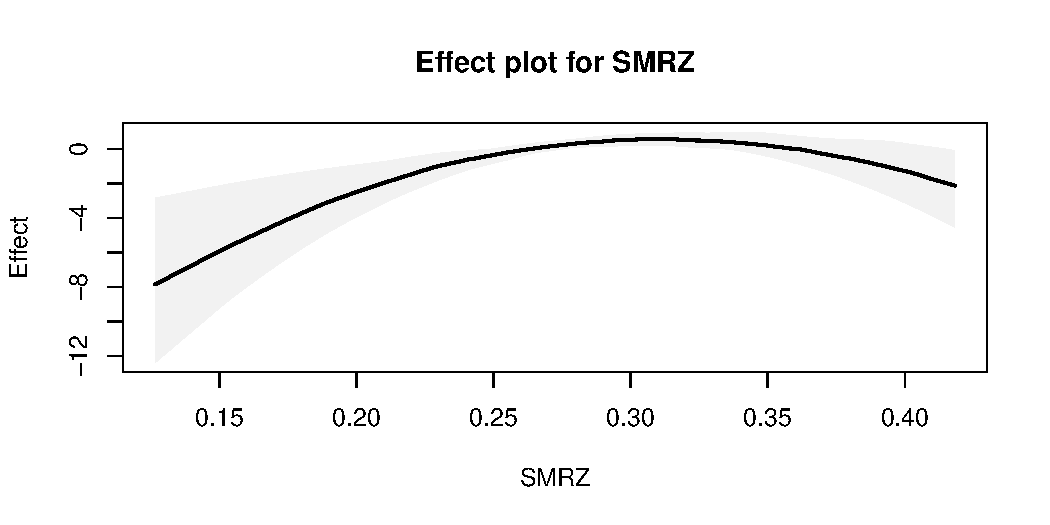
\includegraphics[width=\maxwidth]{figure/interp-1} 

}

\caption[Relationship with Soil Moisture (SMRZ)]{Relationship with Soil Moisture (SMRZ). Black solid line is the median relationship and grey shaded area is the 95 percent CI.}\label{fig:interp}
\end{figure}

\end{knitrout}

\subsection*{DIY Extensions}

Whilst flexible, the \texttt{RISDM} package, and in particular the \texttt{isdm} function, do not cover the full dazzling variety of models that can be fitted using \texttt{INLA}. This is intentional as it keeps the syntax cleaner and learning curve less step. However, many extensions of the ISDM approach will require solving the same set of problems that \texttt{RISDM} handles. For this reason, advanced users may wish to use \texttt{RISDM} as a component for their workflow. \texttt{RISDM} will handle building the \texttt{INLA} stacks for multiple data sources and building the multiple likelihood structures.

To enable this, the \texttt{isdm} function returns some useful data objects. Top of this list is the \texttt{INLA} data stack, held in the `stack' element of the object list. Also useful is the return of the \texttt{INLA} object itself, held in the `mod' object of the object list. These are accessed from, for example, \texttt{fm\$stack} and \texttt{fm\$mod}.

\subsection*{Single Data Types}

Whilst created with multiple data types in mind, \texttt{RISDM} will quite happily estimate models based on single data types too. We'll do this now for a bit of comparative `fun'. The fits produce numerical issues (see output), which should be investigated and corrected for in a real analysis setting. However, to demonstrate the mechanics of fitting single data type models they are \textit{almost} ignorable. In part, their existance supports the thesis that combining data can produce more information and better models than any single species model. If the warnings weren't present, then these models and predictions could be compared against the integrated model (e.g. Figure \ref{fig:pred}).

\begin{knitrout}
\definecolor{shadecolor}{rgb}{0.969, 0.969, 0.969}\color{fgcolor}\begin{kframe}
\begin{alltt}
\hlcom{#PO data only}
\hlstd{fm.PO} \hlkwb{<-} \hlkwd{isdm}\hlstd{(} \hlkwc{observationList}\hlstd{=}\hlkwd{list}\hlstd{(} \hlkwc{POdat}\hlstd{=gamba_PO),}
            \hlkwc{covars}\hlstd{=covars,}
            \hlkwc{mesh}\hlstd{=my.mesh,}
            \hlkwc{responseNames}\hlstd{=}\hlkwa{NULL}\hlstd{,}
            \hlkwc{sampleAreaNames}\hlstd{=}\hlkwa{NULL}\hlstd{,}
            \hlkwc{distributionFormula}\hlstd{=}\hlopt{~}\hlnum{0}\hlopt{+}\hlkwd{poly}\hlstd{( DEM,} \hlnum{2}\hlstd{)} \hlopt{+} \hlkwd{poly}\hlstd{( SMRZ,}\hlnum{2}\hlstd{)} \hlopt{+} \hlstd{ACC,}
            \hlkwc{biasFormula}\hlstd{=}\hlopt{~}\hlnum{1}\hlopt{+}\hlstd{ACC,}
            \hlkwc{artefactFormulas}\hlstd{=}\hlkwa{NULL}\hlstd{,}
            \hlkwc{control}\hlstd{=}\hlkwd{list}\hlstd{(} \hlkwc{coord.names}\hlstd{=}\hlkwd{c}\hlstd{(}\hlstr{"x"}\hlstd{,}\hlstr{"y"}\hlstd{),}
                          \hlkwc{int.sd}\hlstd{=}\hlnum{1000}\hlstd{,} \hlkwc{other.sd}\hlstd{=}\hlnum{10}\hlstd{,} \hlkwc{prior.mean}\hlstd{=}\hlnum{0}\hlstd{,}
                          \hlkwc{prior.range}\hlstd{=}\hlkwd{c}\hlstd{(}\hlnum{1}\hlstd{,}\hlnum{0.1}\hlstd{),} \hlkwc{prior.space.sigma}\hlstd{=}\hlkwd{c}\hlstd{(} \hlnum{5}\hlstd{,}\hlnum{0.1}\hlstd{)))}
\hlstd{fm.PO}\hlopt{$}\hlstd{preds} \hlkwb{<-} \hlkwd{predict}\hlstd{( fm.PO,} \hlkwc{covars}\hlstd{=covars,} \hlkwc{S}\hlstd{=}\hlnum{50}\hlstd{,}
                       \hlkwc{intercept.terms}\hlstd{=}\hlstr{"PO_Intercept"}\hlstd{)}
\hlkwd{plot}\hlstd{( fm.PO}\hlopt{$}\hlstd{preds}\hlopt{$}\hlstd{field)}
\end{alltt}
\end{kframe}\begin{figure}

{\centering 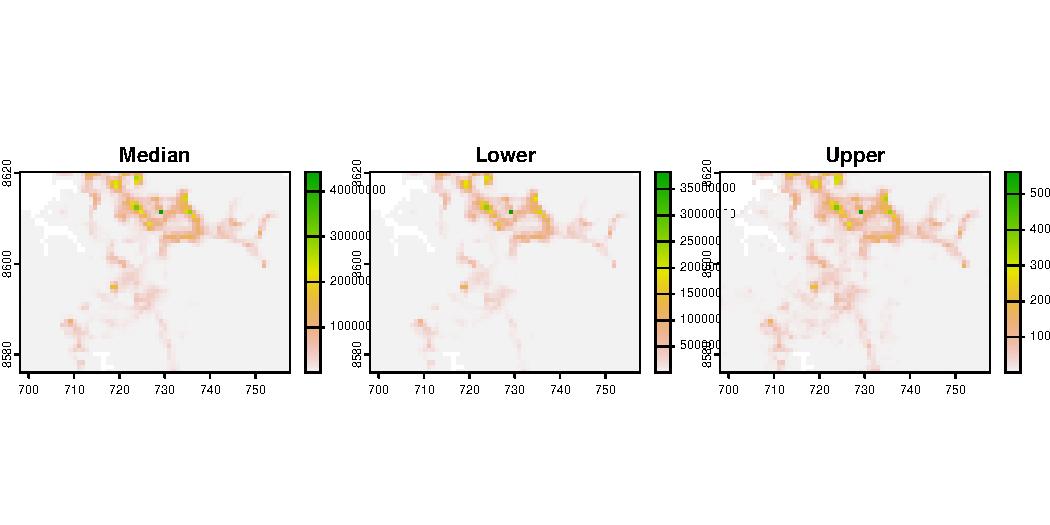
\includegraphics[width=\maxwidth]{figure/singleDataPO-1} 

}

\caption[Intensity model and predictions from estimation using only PA data]{Intensity model and predictions from estimation using only PA data.}\label{fig:singleDataPO}
\end{figure}

\end{knitrout}

\begin{knitrout}
\definecolor{shadecolor}{rgb}{0.969, 0.969, 0.969}\color{fgcolor}\begin{kframe}
\begin{alltt}
\hlcom{#PA data only}
\hlstd{fm.PA} \hlkwb{<-} \hlkwd{isdm}\hlstd{(} \hlkwc{observationList}\hlstd{=}\hlkwd{list}\hlstd{(} \hlkwc{PAdat}\hlstd{=gamba_PA),}
            \hlkwc{covars}\hlstd{=covars,}
            \hlkwc{mesh}\hlstd{=my.mesh,}
            \hlkwc{responseNames}\hlstd{=}\hlkwd{c}\hlstd{(} \hlkwc{PA}\hlstd{=}\hlstr{"PA"}\hlstd{),}
            \hlkwc{sampleAreaNames}\hlstd{=}\hlkwd{c}\hlstd{(} \hlkwc{PA}\hlstd{=}\hlstr{"Area"}\hlstd{),}
            \hlkwc{distributionFormula}\hlstd{=}\hlopt{~}\hlnum{0}\hlopt{+}\hlkwd{poly}\hlstd{( DEM,} \hlnum{2}\hlstd{)} \hlopt{+} \hlkwd{poly}\hlstd{( SMRZ,}\hlnum{2}\hlstd{)} \hlopt{+} \hlstd{ACC,}
            \hlkwc{artefactFormulas}\hlstd{=}\hlkwd{list}\hlstd{(} \hlkwc{PA}\hlstd{=}\hlopt{~}\hlnum{1}\hlstd{),}
            \hlkwc{control}\hlstd{=}\hlkwd{list}\hlstd{(} \hlkwc{coord.names}\hlstd{=}\hlkwd{c}\hlstd{(}\hlstr{"x"}\hlstd{,}\hlstr{"y"}\hlstd{),}
                          \hlkwc{int.sd}\hlstd{=}\hlnum{1000}\hlstd{,} \hlkwc{other.sd}\hlstd{=}\hlnum{10}\hlstd{,} \hlkwc{prior.mean}\hlstd{=}\hlnum{0}\hlstd{,}
                          \hlkwc{prior.range}\hlstd{=}\hlkwd{c}\hlstd{(}\hlnum{1}\hlstd{,}\hlnum{0.1}\hlstd{),} \hlkwc{prior.space.sigma}\hlstd{=}\hlkwd{c}\hlstd{(} \hlnum{5}\hlstd{,}\hlnum{0.1}\hlstd{)))}
\end{alltt}
\begin{verbatim}
Error in inla.inlaprogram.has.crashed() : 
  The inla-program exited with an error. Unless you interupted it yourself, please rerun with verbose=TRUE and check the output carefully.
  If this does not help, please contact the developers at <help@r-inla.org>.

 *** inla.core.safe:  inla.program has crashed: rerun to get better initial values. try=1/2 

 *** inla.core.safe:  rerun with improved initial values 
\end{verbatim}
\begin{alltt}
\hlstd{fm.PA}\hlopt{$}\hlstd{preds} \hlkwb{<-} \hlkwd{predict}\hlstd{( fm.PA,} \hlkwc{covars}\hlstd{=covars,} \hlkwc{S}\hlstd{=}\hlnum{50}\hlstd{,}
                       \hlkwc{intercept.terms}\hlstd{=}\hlstr{"PA_Intercept"}\hlstd{)}
\hlkwd{plot}\hlstd{( fm.PA}\hlopt{$}\hlstd{preds}\hlopt{$}\hlstd{field)}
\end{alltt}
\end{kframe}\begin{figure}

{\centering 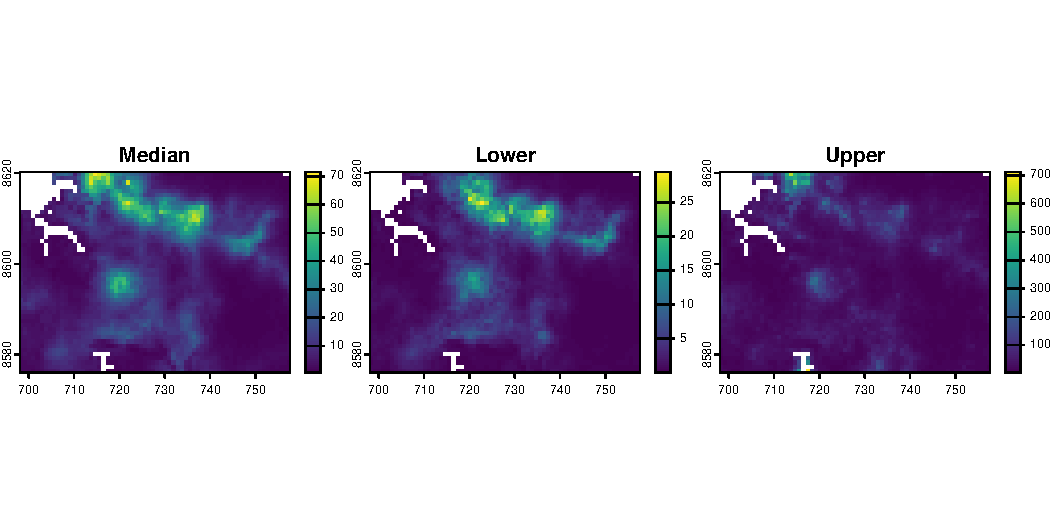
\includegraphics[width=\maxwidth]{figure/singleDataPA-1} 

}

\caption[Intensity model and predictions from estimation using only PA data]{Intensity model and predictions from estimation using only PA data.}\label{fig:singleDataPA}
\end{figure}

\end{knitrout}
  
\section*{Last Things Last}
  
The only remaining thing to do is to tidy up our workspace. This is just removing all objects for this analysis from your workspace. I like to do this, in tutorial situations, but you may not. It is entirely up to you whether you clean or not.
\begin{knitrout}
\definecolor{shadecolor}{rgb}{0.969, 0.969, 0.969}\color{fgcolor}\begin{kframe}
\begin{alltt}
\hlcom{#You may wish to tidy your workspace.}
\hlkwd{rm}\hlstd{( covars, fm, fm.noRand, fm.PA, fm.PO, gamba_PA, gamba_PO, filenames,}
             \hlstd{my.biasForm, my.form, my.control, my.mesh, my.mesh.bad)}
\end{alltt}
\end{kframe}
\end{knitrout}

\section*{Acknowledgements}

This work was partially funded by the Australian Government Department of Agriculture, Fisheries and Forestry’s Established Pest Animals and Weeds Management Pipeline Program and Supporting Communities Manage Pests and Weeds Program.
    
\bibliography{./RISDM}

\section*{Appendix}
  
\subsection*{Computational details}
This vignette was created using the following R and add-on package versions
  
\begin{itemize}\raggedright
  \item R version 4.2.1 (2022-06-23), \verb|x86_64-pc-linux-gnu|
  \item Locale: \verb|LC_CTYPE=en_AU.UTF-8|, \verb|LC_NUMERIC=C|, \verb|LC_TIME=en_AU.UTF-8|, \verb|LC_COLLATE=en_AU.UTF-8|, \verb|LC_MONETARY=en_AU.UTF-8|, \verb|LC_MESSAGES=en_AU.UTF-8|, \verb|LC_PAPER=en_AU.UTF-8|, \verb|LC_NAME=C|, \verb|LC_ADDRESS=C|, \verb|LC_TELEPHONE=C|, \verb|LC_MEASUREMENT=en_AU.UTF-8|, \verb|LC_IDENTIFICATION=C|
  \item Running under: \verb|Ubuntu 20.04.6 LTS|
  \item Matrix products: default
  \item BLAS:   \verb|/usr/lib/x86_64-linux-gnu/blas/libblas.so.3.9.0|
  \item LAPACK: \verb|/usr/lib/x86_64-linux-gnu/lapack/liblapack.so.3.9.0|
  \item Base packages: base, datasets, graphics, grDevices, methods,
    stats, utils
  \item Other packages: knitr~1.39, raster~3.6-3, RISDM~1.2.9, sp~1.6-0
  \item Loaded via a namespace (and not attached): codetools~0.2-18,
    colorRamps~2.3, compiler~4.2.1, deldir~1.0-9, evaluate~0.21,
    foreign~0.8-82, grid~4.2.1, highr~0.8, INLA~23.04.24,
    lattice~0.20-45, magrittr~2.0.3, maptools~1.1-5, Matrix~1.5-3,
    MatrixModels~0.5-1, mnormt~2.0.2, numDeriv~2016.8-1.1,
    parallel~4.2.1, Rcpp~1.0.10, rgdal~1.5-32, rgeos~0.5-9, sn~2.1.1,
    splancs~2.01-40, splines~4.2.1, stats4~4.2.1, stringi~1.5.3,
    stringr~1.4.0, terra~1.7-29, tmvnsim~1.0-2, tools~4.2.1, xfun~0.31
\end{itemize}

    
\end{document}
  
